\documentclass{if-beamer}

% --------------------------------------------------- %
%                  Presentation info	              %
% --------------------------------------------------- %
\title[Modulador]{Modulador Para El amplificador clase D}
\subtitle{Universidad ICESI}
\author{M. Gallego. R, \\
N. J. Salazar. E.}
\institute[ICESI]{
}
\date{\today}
\logo{

\includegraphics[scale=0.080]{figuras/ICESI.jpeg}
}
\subject{Presentation subject} % metadata

\graphicspath{{figuras/}}
% --------------------------------------------------- %
%                    Title + Schedule                 %
% --------------------------------------------------- %

\begin{document}

\begin{frame}
  \titlepage
\end{frame}

\begin{frame}{Contenido}
  \tableofcontents
\end{frame}

% --------------------------------------------------- %
%                      Presentation                   %
% --------------------------------------------------- %
%%%%%%%%%%%%%%%%%%%%%%%%%%%%%%%%%%%%%%%%%%%%%%%%%%%%%%%
%%%%%%%%%%%%%%%%%%%%%%%INTRODUCCCIÓN%%%%%%%%%%%%%%%%%%%
%%%%%%%%%%%%%%%%%%%%%%%%%%%%%%%%%%%%%%%%%%%%%%%%%%%%%%%
\section{Introducción}
\subsection{¿Qué es una modulación?}
\begin{frame}{¿Qué es una modulación?}

Es la modificación de un parametro de la señal por otra, este 
párametro puede ser frecuencia, amplitud, fase, los elementos que hacen parte de la modulación son: 

\begin{itemize}
    \item \textbf{señal portadora: } Es la señal encargada de transportar la información su frecuencia es la frecuencia de transmisión 
    \item \textbf{Señal moduladora: } Es la señal que contiene la información 
    \item \textbf{Señal modulada: } Es la señal que resulta de la modulación 
\end{itemize}{}
\end{frame}{}

\subsection{¿Qué es el muestreo?}
\begin{frame}{¿Qué es el muestreo?}
\begin{center}
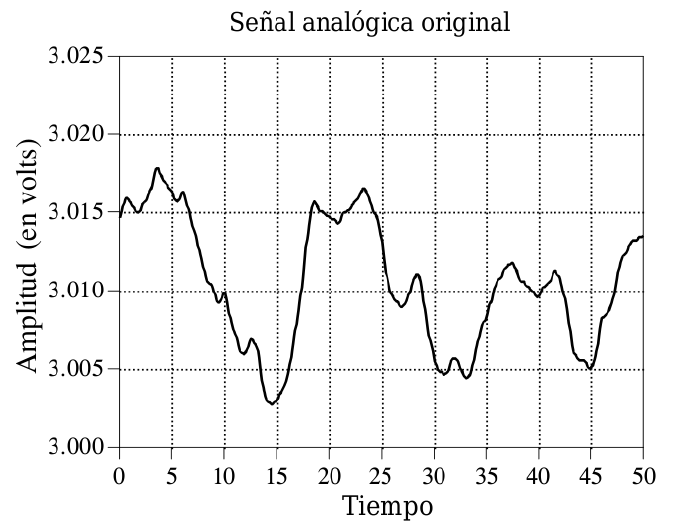
\includegraphics[scale=0.40]{figuras/senal.png}
\end{center}{}
\end{frame}{}

\begin{frame}{}
\begin{center}
    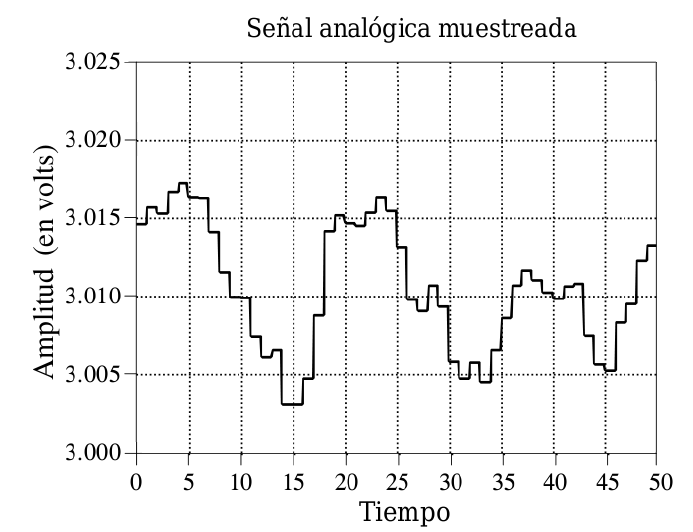
\includegraphics[scale=0.4]{figuras/senal2.png}
\end{center}{}
    
\end{frame}{}

\subsection{Modulación PWM}
\begin{frame}{Modulación PWM (modulación por duración de pulso)}
   
    
    \begin{center}
        \includegraphics[scale=0.8]{figuras/imagen2.jpeg}
    \end{center}{}
    
\end{frame}{}
%%%%%%%%%%%%%%%%%%%%%%%%%%%%%%%%%%%%%%%%%%%%%%%%%%%%%%%
%%%%%%%%%%%%%%%%%%%%%%IMPLEMENTACIÓN%%%%%%%%%%%%%%%%%%%
%%%%%%%%%%%%%%%%%%%%%%%%%%%%%%%%%%%%%%%%%%%%%%%%%%%%%%%
\section{Implementación del Modulador}

\subsection{Materiales}

\begin{frame}{Materiales}
    \begin{center}
        \begin{itemize}
            \item Amplificador operacional LF353
            \item Protoboard 
            \item Cables macho-macho
            \item Arduino uno (fuente alimentación)
            \item Analog Discovery
        \end{itemize}{}
    \end{center}{}    
        
\end{frame}{}

\subsection{Montaje}
\begin{frame}{Montaje}

\begin{center}
    \includegraphics[scale=0.4]{figuras/fritzing1.png}
\end{center}{}

\end{frame}{}

\subsection{Resultados}
\begin{frame}{Resulatdos}
    \begin{center}
    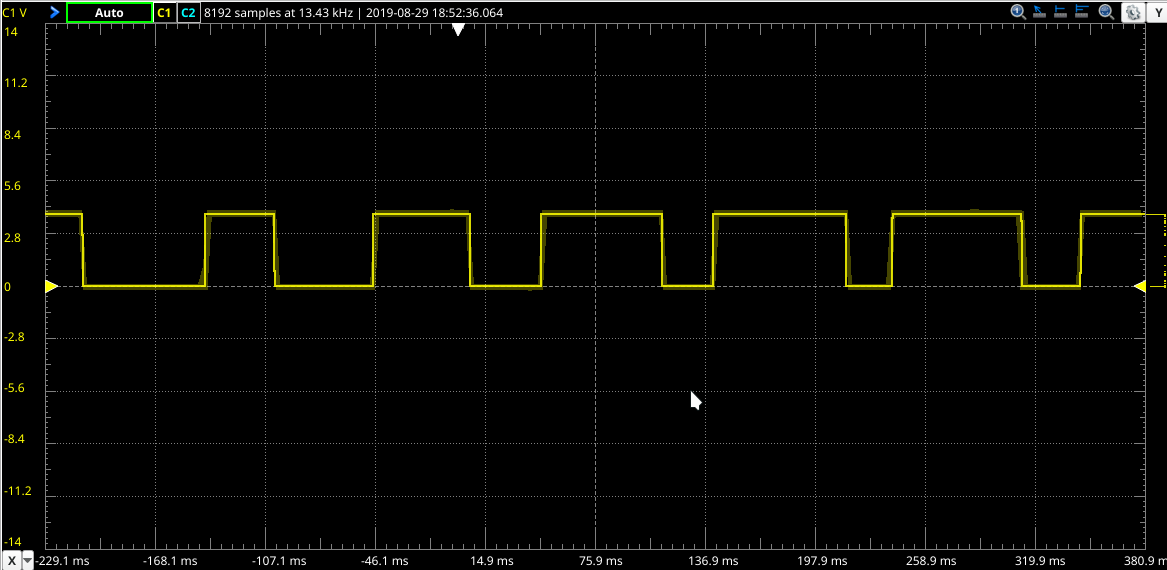
\includegraphics[scale=0.3]{figuras/modulacion1.png}
\end{center}{}
\end{frame}{}

\section{Conclusiones}
\begin{frame}{Conclusiones}
\begin{itemize}
    \item ruido
    \item relaciones: amplitud-ruido, frecuencia-ruido
    \item PWM = analogica 
    
\end{itemize}{}

\end{frame}{}

\section{Preguntas}


\end{document}
